\pagestyle{headings}

\chapter{Introduction}

\pagenumbering{arabic} 
\setcounter{page}{8}

\section{Motivation}

How much am I paying due to the energy consumption of my fridge? While simple, a typical homeowner do not have access to this kind of information yet. Providing energy usage feedback to homeowners is a helpful way for promoting the energy efficiency \cite{eci}. Detailed information on energy consumption is still invisible to the general population which implies in a source of waste. Without feedback, it is impossible for people to learn effectivelly about their energy usage patterns, necessary for energy savings. Unlike phone bills in which calls are individually identified, the energy bill shows only the total price which is a limited information. 

As shown in the Fig.~\ref{feedback}, the energy feedback can be either indirect or direct \cite{epri}. As a difference, the indirect feedback is provided after the consumption occurs which may range from a standard electricity bill to daily reports. The direct feedback, on the other hand, is provided in real time with either aggregated or disaggregated real-time energy usage information. The later one means appliance level information regarding the energy consumption and operating state, which is the focus of this work. Disagregated real-time feedback is a valuable resource for homeowners, commercial buildings, and power utilities. For homeowners and commercial buildings, disaggregation helps them making decisions about their consumption habits and appliances to save energy \cite{CarrieArmel2013213}. In addition, it can be helpful to detect malfunctions, inefficient equipment or for scheduling predictive maintenance \cite{eunilm2016}. In regards to power utilities, disaggregation helps them to understand their customers and provide them with better-customized services \cite{eunilm2016-2}. 

The disaggregation of loads can be accomplished either with intrusion or not intrusively. In an intrusive approach, it is necessary to connect one measurement device to each power outlet, which leads to high installation costs and privacy concerns. On the non-intrusive approach, the energy consumption of the major appliances is estimated using only a single meter installed in the consumer’s energy input panel. The measurements acquired by the energy meter are processed in order to provide details about the operating devices. The advantage of non-intrusive identification is the reduced costs of hardware, maintenance, and privacy. However, non-intrusive identification is still a software challenge due to the complexity of extracting a set of source signals from a mixed signal. This challenge is closely related to the cocktail party problem where there are multiple sound sources recorded by a microphone and we want to extract just one of these sources \cite{ica}. In this context, the objective of non-intrusive load monitoring (NILM), also known as load disaggregation, is to break down a whole-home power signal into individual devices.

\begin{figure}[tb]
    \centering
    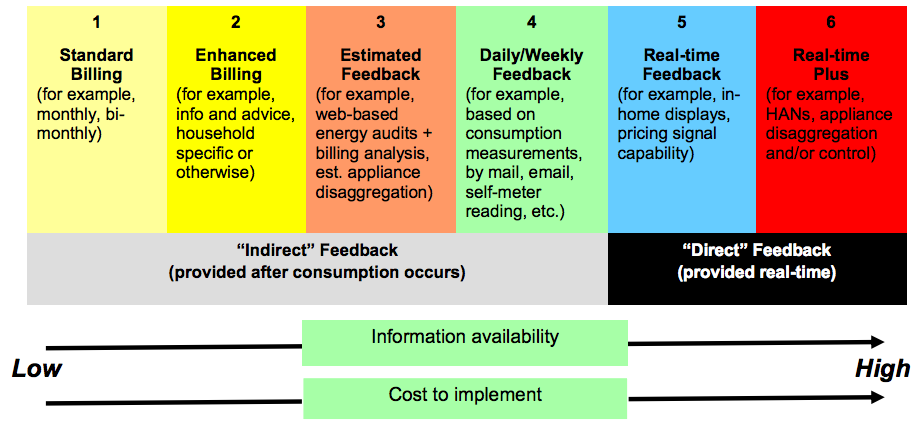
\includegraphics[width=1\columnwidth ]{feedback.png}
    \caption{Spectrum with the different types of energy feedback (Source: \cite{epri})}
    \label{feedback}
\end{figure}

\iffalse
How much energy did my fridge spend in the last month? While simple, a typical homeowner still do not have access to this kind of information. The number of energy meters in the world is expected to increase up to 780 Million by 2020 \cite{first}. However, unlike phone bills in which calls are individually identified and marked, the energy bill shows only the total price. No information about the consumption of each appliance is provided. Disaggregation of loads from power measurements is a valuable resource for homeowners, commercial buildings, and power utilities. For homeowners and commercial buildings, disaggregation helps them making decisions about their consumption habits and appliances to save energy \cite{CarrieArmel2013213}. In addition, it can be helpful to detect malfunctions, inefficient equipment or for scheduling predictive maintenance \cite{eunilm2016}. In regards to power utilities, disaggregation helps them to understand their customers and provide them with better-customized services \cite{eunilm2016-2}. The disaggregation of loads can be accomplished either with intrusion or not intrusively. In an intrusive approach, it is necessary to connect one measurement device to each power outlet, which leads to high installation costs and privacy concerns. On the non-intrusive approach, the energy consumption of the major appliances is estimated using only a single meter installed in the consumer's energy input panel. The advantage of non-intrusive identification is the reduced costs of hardware, maintenance, and privacy. In this context, the objective of non-intrusive load monitoring (NILM), also known as load disaggregation, is to break down a whole-home power signal into individual appliances.
\fi

\section{Description of the Problem}

The keyword NILM\footnote{Nowadays, this keyword have also extended to equivalents NIALM (non-intrusive appliance load monitoring) and NALM (nonintrusive appliance load monitoring). Another commonly and equivalent keyword is load disaggregation.} was introduced in 1985 by George W. Hart in a technical report \cite{hart85} and later published in 1992 by the same author \cite{hart}. The paper proposes a full methodology, from types of loads, load signatures, algorithm and physical implementation. The algorithm is based in the context of a communication model where each appliance is a 'transmitter' and the algorithm is modeled as a 'receiver'. The author then proposes a 'decoding'  algorithm. 

The algorithm is based on event (edge) detection. Then, it groups these events into clusters of active and reactive power. The next step is to construct appliance models. Next, single state appliances are identified by clustering pair of events. As advantage, this algorithm works even in an unsupervised way, where it clusters similar events and then tracks the following events based on their proximity. Another advantage is that this algorithm works well even in the presence of unknown appliances. As disadvantage, since this method is solely based on event detection, it might miss some event due to a case where multiple events occur. Another common problem is that in case a off and the immediately following on event are both missed. The algorithm connects the previous ON with the subsequent ON event. 

However, before introducing the pattern recognition method, Hart describes the NILM problem as a combinatorial optimization (CO) problem. In the CO formulation, the disaggregation is obtained by combining the multiple possible states that minimizes the full measurement for each time instant. For each time instant, we seek to minimize the combination of power states and the final measurement. Here, it is assumed that all the possible operating states are previously known. Hart points three main issues to discourage the usage of this formulation. The first issue is that we have a NP-complete “weighted set” problem, hence it has a high computational cost and it increases with the addition of more states of devices or measurements. The second problem - mentioned as the 'fundamental problem' - is that the complete set of operating states are never known. If the model is used in the presence of unknown appliances, it would attempt to describe their behavior as a combination of other known appliances. Finally, the third problem - which will be referred as the multiple switching (MS) problem - is that a small change in the measurement might be translated in a big change of the combination of loads. Despite various NILM approaches proposed in the literature, the next section shows that very few have attempted in dealing with those problems. As shown in later sections, this work is going to explore the potential of expanding the CO formulations in ways to handle the previous problems. We are especially concerned in solving the MS problem. New constraints could be proposed for this purpose. In addition, methods can be explored to decrease the running time. 


\iffalse


, formulated in the following way: let's assume that the measured value (current/power) in the input of the house is $P(t)$ at time $t$. The goal of the algorithm would be to decode $P(t)$ in many components $P_i(t) \ \forall \ i \in 1..n$, where $n$ is the number of power components and each one would be be associated to one specific state $i$. Hence, we have that

$$P(t) = P_1(t) + ... + P_n(t)$$
 
The CO formulation can be written by using the equation \ref{co} for each time reading $t$ 

\begin{equation} \label{co}
    \min_{x} \quad \left|P(t) - \sum_{i=1}^{n} x_i\ P_i \right|
\end{equation}

where $x_i(t)$ is a boolean that describes the state of the power component $i$ at time $t$. As noted in the reference, this problem although mathematically attractive, is a NP-complete “weighted set” problem, hence it has a high computational cost. In addition, it's complexity increases with the addition of more states of devices or measurements.
Hart's paper points to a few difficulties in estimating $x_i(t)$. The first - mentioned as the 'fundamental problem' - is that the complete set of $P_i$ are never known. As disadvantage, if the model is used in the presence of unknown appliances, it would attempt to describe their behavior as a combination of other known appliances. 
The second difficulty is that a small change in $P(t)$ might be translated in a big change of the combination of loads. Despite various NILM approaches proposed in the literature, the literature review in the next section shows that very few have attempted in dealing with those problems. While the two difficulties are quite challenging in both accuracy and running time, there is still room for improvements. 

\fi

\section{Previous work}

Figure \ref{1npub} shows the number of publications in the NILM field per year over the last 25 years. Those NILM publications are inferred using publications citing the first NILM work published by Hart in 1992\footnote{Inspired from \cite{1npub}. Data acquired from Google Scholar. Code available in \url{https://github.com/WittmannF/nilm-publications}}. An exponential growth of NILM publications can be observed since 2010.

\begin{figure}[bt]
    \centering
    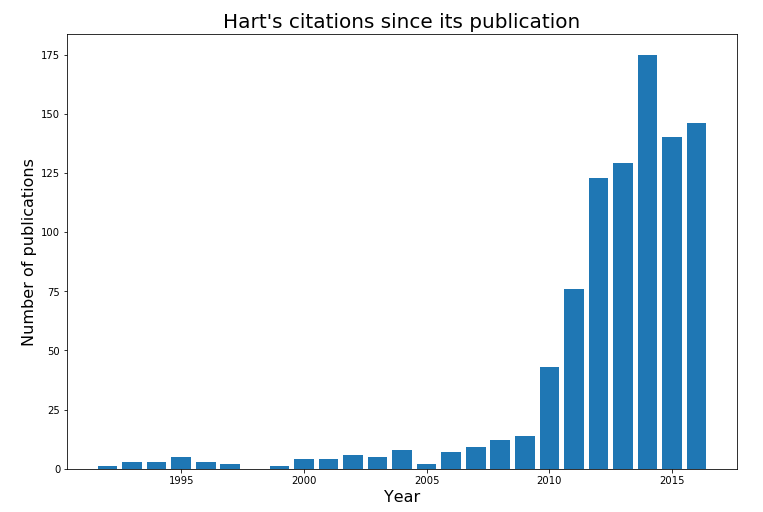
\includegraphics[width=0.8\textwidth]{npub}
    \caption{Number of publications with reference to Hart's original work since its publication}
    \label{1npub}
\end{figure}


%The second problem led the author to propose the switch continuity principle (SCP), which states: \textit{``In a small time interval, we expect only a small number of appliances to change state in a typical load''}. However, as shown in recent works \cite{makonin2016}, SCP is not always reliable. Hence, a better strategy to deal with MS is necessary.
A further analysis in the publication's titles since 2010 did not reveal any trending strategy. Figure \ref{wordle} shows the most frequent words that were found in those titles. Some obvious keywords such as 'nonintrusive', 'load', 'monitoring', 'energy' and 'disaggregation' were removed. As main insights, the NILM research field seems to be mainly focused in residential applications and buiding. Therefore, few attention has been paid to industrial applications. In addition, it seems that privacy is increasingly a concern in the field. Another analysis using only the split of the title after the keyword 'based on' and 'using' was also considered. However, this analysis did not reveal too much insight of key techniques as well. 

\begin{figure}[bt]
    \centering
    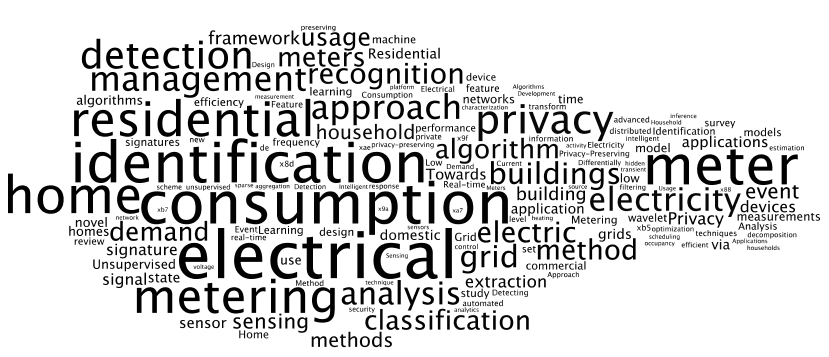
\includegraphics[width=0.8\textwidth]{wordle}
    \caption{Trending words in NILM publications since 2010}
    \label{wordle}
\end{figure}

- There are many ways of categorizing the NILM approaches. 
- For example they can be categorized into either supervised or unsupervised approaches. In the NILM supervised approach, it is assumed the access to the measurements of each single appliance for training a disaggregation algorithm. In the NILM unsupervised approach, 
- Zeifman and Roth in \cite{zeifman} divide the types of algorithms in two categories: pattern recognition (one-to-one matching) and optimization (multiple matching).
- Nowadays, Zeifman's categorization can be expanded into either event based algorithms or eventless algorithms. 

The pattern recognition matching is based on the detection and classification of events. Since the pattern recognition strategies are based on one-to-one matching, the efforts of these strategies are mainly focused on feature extraction. These events are then classified by well-established classifiers, such as k-nearest neighbor \cite{Figueiredo2011}, \cite{berges2009, Froehlich2010}, fuzzy sets \cite{lin2011, ducange2014}, decision trees \cite{Nguyen2015, gillis2016}, support vector machines \cite{duarte2012, zoha2012}, neural networks \cite{zhou2016, bian2016} and deep learning \cite{mauch2016, jack2015}. As noted by \cite{zeifman}, the advantages of pattern recognition methods are that they provide better results in the presence of unknown loads. However, those methods are sensible to the detection of false edges coming from noise or non-linear loads.

On the other hand, optimization methods are based on the simultaneous matching of multiple loads, and they find the set of energized appliances that best fit the measured load. Most efforts from researchers on this side are given methods based on hidden Markov models (HMM) \cite{afhmm, reed, hmm_unsup, stephen_hmm}. Other approaches includes sparse coding \cite{sparse_kolter, nmf}, genetic algorithms \cite{meta} and integer programming \cite{suzuki, bhotto2016}. These optimization methods provide better disaggregation performance \cite{zeifman} and are less sensible to edge detection. However, they are more susceptible to the MS and FP problem.

Regarding the optimization approaches, very few of them were focused on expanding the classical CO model. Some of these works are going to be discussed next. Egarter and Elmenreich in \cite{meta} verify the MS problem by evaluating six meta-heuristics to solve the CO problem formulated as a knapsack problem. 

Kolter and Jaakkola in \cite{afhmm} formulate the NILM problem as a convex quadratic programming problem. The authors consider an extension to HMMs, called additive factorial hidden Markov models. Furthermore, authors in \cite{afhmm} describe an unsupervised learning procedure. However, the method needs a regularization parameter that changes for each problem. In addition, the optimization function is made over the full set of time periods, which make the method computationally expensive.


Authors in \cite{suzuki} formulate the NILM problem as an integer quadratic programming problem. The technique use in \cite{suzuki} represents the NILM problem as a combination of multiple currents. As a drawback, the model is based on the reading of one AC cycle (total waveform), so a large number of samples in high sampling rate is required.

Finally, authors in \cite{bhotto2016} propose a load disaggregation method based on integer linear programming. The work proposes enhancements to CO, such as state transition diagram and median filtering, to deal with the MS. Most enhancements in \cite{bhotto2016} are included as an intensive preprocessing rather than constraints. In addition, the model does not include the set of time periods in the optimization function. Hence, their model is limited to the usage of constraints that does not depend on time measurements.



 Yumoto suggested a method based on Neural Network (NN) whose inputs are higher harmonic spectrum in order to identify electronic appliances. Murata suggested a method in which Hart's method is combined with to NN. Nakamura suggested a method based on Hidden Markov Model (HMM). This method models the current waveforms and estimates the operating conditions. Nowadays they can be divided in either a supervised or unsupervised approach. In the supervised approach, previous knowledge about appliances is used. In the unsupervised, no previous knowledge is necessary. Some examples of algorithms for unsupervised are clustering and FMM. Most methods are focused on using machine learning techniques such as deep neural networks, ensembles and clustering. These methods might leads to practical solutions when there is a large and representative database available, which is not always the case. There are some popular datasets such as REED, X and Z, however they still represents only a small slice of the variability present. Alternative approaches includes combinatorial optimization, also know as integer programming (IP) is still an emerging technique to be explored. Some notables works will be seen next. 

\subsection{Optimization Related Work}
Three previous works were found using optimization techniques and are going to be presented here. \cite{suzuki} formulates the NILM problem as an integer quadratic programming problem. The technique represents the problem, as a combination of sums of the current of multiple loads. 
At any given one period of current, the overall load current is represented as a superposition of each current of the operating appliance. This is true since the overall current waveform is highly influenced by the waveform of each individual appliance. Each of them has their own properties as shown in the example of Figure \ref{1suzuki}. As advantage, the model considers cases with multiple modes and also same-type operating simultaneously. As limitation, it requires very high frequency data. The model is based on the reading of one cycle (60Hz or 50Hz), so a large number of points from each cycle is necessary.


\begin{figure}
    \centering
    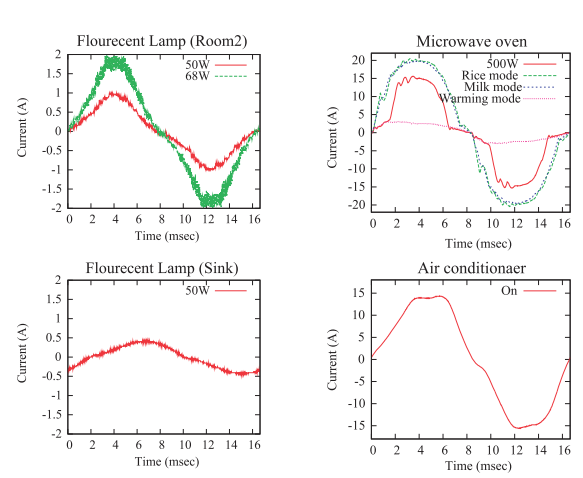
\includegraphics[width=0.8\textwidth]{1suzuki}
    \caption{Example of current waveforms for different loads, used by \cite{suzuki}}
    \label{1suzuki}
\end{figure}


\cite{meta} shows the classic problem pointed in Hart's paper and discusses their equivalency with the knapsack problem. In short, it states that the classic equation is equivalent to the knapsack problem presented in \ref{knap} with a profit d of 1 for all loads, and considering the capacity C corresponds to the total load $P(t)$. However this paper is focused on verifying Hart’s statement regarding the Switch Continuity Principle. 5 metaheuristics optimization approaches are tested and  and does not deepen on the appliance model. No additional constraint is considered in order to enhance the identification accuracy. It concludes that it is hard to disaggregate loads with power drawns.
Finally is proposes as future work a multi-objective optimization approach employing multiple features such as reactive power, common time of usage and common duration time.

\begin{equation} \label{knap}
   max \quad \sum_{i=1}^{n} d_i \ x_i
\end{equation}

$$ s. \ t. \quad \sum_{i=1}^{n} w_i \ x_i \leq C $$

\cite{stephen} proposes a load disaggregation method based on aided linear integer programming. It enhances the work done on \cite{suzuki} by rewriting as a linear programming problem, including additional constraints, correction based on a state diagram, and median filtering. As advantage, the proposed technique does not requires waveform signatures as in the other work since it relies only on instantaneous load samples. 

This work was initially looking to replicate \cite{stephen} and evaluate possible improvements. It end up following a different path due to the difference of languages, although many of the insights where very helpful. Equivalent strategies to the state transition diagram and median filtering are going to be presented here, however using a different and novel approach. In addition, an automatic appliance state extraction method is presented on the Appendix. 


The first NILM technique was published by Hart \cite{hart} in 1992 using a pattern recognition approach. The technique is based on event detection and grouping those events into clusters of active power and reactive power features. 

\section{Objectives}

Based on the efforts made by previous works, the goal of this paper is to represent and solve the NILM problem as a mixed-integer linear programming (MILP) problem. We are especially concerned on dealing with the MS problem and compare with other methods based on pattern recognition and CO.

%The contributions of this work are brought from (). The work deals with the unit commitment problem in which try to allocate multiple combination of termal units for a given period. The constraints for modeling time and x demonstrates to be useful for NILM . 

\section{Contributions}

The main contributions of this paper are as follows:

\begin{itemize}
\item The NILM problem is represented as a MILP model, in which a new set of integer linear constraints is proposed to efficiently model the load signatures of the appliances.
\item In order to enhance the computational performance, the proposed NILM is solved using a window-based algorithm in which the overall problem is segmented into small, coupled sub-problems that can be efficiently solved via commercial MILP solvers.
\item The proposed model is also suitable for unsupervised NILM in the context described in \cite{makonin2016}. The model relies in parameters that can be acquired from aggregated data, such as, minimum operation time and sequence of states.
%\item A new set of constraints to model the load signature
%\item A window based algorithm in order to make the algorithm to run more efficiently
%\item The problem that led Hart to propose the \textit{switch continuity principle} is avoided in the tests cases
\end{itemize}

\section{Organization of the Work}

The next sections of this dissertation goes in this way:
\begin{itemize}
\item The Chapter 2 describes some background work that is used as basis for the remaining chapters. The reader may skip subsections that are already familiar with. 
\item The Chapter 3 describes the main contributions of this work. A math model for modeling the load signature. 
\item The Chapter 4 describes the process of extracting the features that are used for feeding the input table of the model. The chapter is divided into two subsections: A supervised approach which uses clustering for extracting the main information and an unsupervised approach which is based on edge detection and histogram analysis.
\item The Chapter 5 describes the test cases with results for both the unsupervised setting and the supervised one. 
\item Finally, the Chapter 6 presents the main conclusions and future work. 
\end{itemize}